\documentclass[conference]{IEEEtran}
\IEEEoverridecommandlockouts

\usepackage{cite}
\usepackage{amsmath,amssymb,amsfonts}
\usepackage{graphicx}
\usepackage{booktabs}
\usepackage{listings}
\usepackage{xcolor}
\usepackage{url}
\usepackage{hyperref}
\usepackage[T1]{fontenc}
\usepackage[utf8]{inputenc}
\usepackage[english]{babel}
\usepackage{tikz}
\usetikzlibrary{arrows.meta, positioning, shapes.geometric, fit, backgrounds}

\graphicspath{{images/}}

\hypersetup{
  colorlinks=true,
  linkcolor=black,
  citecolor=black,
  urlcolor=blue,
}

\begin{document}

\title{HantaBERT: Multi-Task Hantavirus Classification\\with DNABERT-2 Fine-Tuning}

\author{%
\IEEEauthorblockN{%
\begin{tabular}{@{}c@{\hspace{2.5em}}c@{\hspace{2.5em}}c@{}}
Muhammad Faiz Atharrahman\textsuperscript{1} &
Muhammad Rafi Dhiyaulhaq\textsuperscript{2} &
Lydia Gracia\textsuperscript{3} \\
18222063 & 18222069 & 18222035
\end{tabular}}
\IEEEauthorblockA{%
Information Systems and Technology Major \\
School of Electrical Engineering and Informatics \\
Institut Teknologi Bandung \\[2pt]
\textsuperscript{1}\texttt{m@faiz.at} \quad$\cdot$\quad
\textsuperscript{2}\texttt{rafidhiyaulh@gmail.com} \quad$\cdot$\quad
\textsuperscript{3}\texttt{ly.gracies@gmail.com}
}
}

\maketitle

\begin{abstract}
Hantaviruses are a group of zoonotic RNA viruses transmitted primarily by
rodents and capable of causing severe hemorrhagic fever in humans.
Rapid classification of a new sequence (covering the virus species, the
likely reservoir host, and its geographic origin) is a crucial step in
outbreak response. This study proposes \emph{HantaBERT}, a multi-task
model obtained by \emph{fine-tuning} the genome foundation model
\textsc{DNABERT-2} on 8{,}822 hantavirus sequences from NCBI GenBank.
The proposed architecture places a shared \emph{bottleneck} on top of the
DNABERT-2 \emph{encoder}, then branches into three independent
classification heads for predicting species (23 classes), host
(3 classes), and geographic origin (7 continents). Training is performed
with a weighted cross-task \emph{loss} $L = 1{.}0\,L_{\text{sp}} + 0{.}5\,L_{\text{host}}
+ 0{.}3\,L_{\text{geo}}$, a differential encoder-vs-head \emph{learning rate},
and memory optimization via \emph{gradient accumulation} + AMP fp16. On a
held-out test set, the model achieves 96{.}7\% accuracy (species), 91{.}4\%
(host), and 80{.}5\% (geography). A UMAP visualization of the
\emph{bottleneck embedding} reveals separation of viral \emph{lineages}
as well as substructure per genome segment ($S$/$M$/$L$) without any
explicit \emph{clustering} objective, indicating the emergence of a
meaningful phylogenetic representation. The code is available at
\url{https://github.com/HantaBERT}.
\end{abstract}

\begin{IEEEkeywords}
hantavirus, DNABERT-2, multi-task learning, nucleotide sequence
classification, genome embedding, UMAP
\end{IEEEkeywords}

% =============================================================================
\section{Introduction}\label{sec:intro}
% =============================================================================

\subsection{Hantavirus Biology Concepts}

Hantaviruses (family \emph{Hantaviridae}, genus \emph{Orthohantavirus})
are negative-sense single-stranded RNA viruses with a tripartite
segmented genome: the \textbf{S} segment (\emph{small}, $\sim$1{.}8 kb)
encodes the nucleocapsid (N) protein that wraps the genome; the
\textbf{M} segment (\emph{medium}, $\sim$3{.}6 kb) encodes a glycoprotein
precursor that is cleaved into the envelope-forming Gn and Gc; and the
\textbf{L} segment (\emph{large}, $\sim$6{.}5 kb) encodes the
RNA-\emph{dependent} RNA polymerase (RdRp). These viruses are transmitted
primarily by rodents, with several species able to cause two severe
clinical syndromes in humans:
\emph{Hantavirus Cardiopulmonary Syndrome} (HCPS) in the Americas and
\emph{Hemorrhagic Fever with Renal Syndrome} (HFRS) in Eurasia.
Rapid identification of new sequences is an important component of
outbreak response and epidemiological surveillance.

\subsection{Related Computational Methods}

Classical approaches based on \emph{alignment} and phylogenetic trees
(\emph{neighbor-joining}, \emph{maximum likelihood}) yield accurate
results but require compute-intensive preprocessing and are sensitive to
the choice of reference region. Deep learning approaches offer an
alternative path: \emph{Convolutional Neural Networks} (CNNs) for viral
taxonomic classification and, more recently, Transformer foundation
models for nucleotide sequences. \textsc{DNABERT}~\cite{Ji2021DNABERT}
trains a BERT \emph{encoder}~\cite{Devlin2019BERT} on the human genome
with $k$-\emph{mer} tokenization;
\textsc{DNABERT-2}~\cite{Zhou2023DNABERT2} extends it to multiple species
with a more efficient \emph{Byte-Pair Encoding} tokenization;
\textsc{DNABERT-S}~\cite{Zhou2024DNABERTS} adds a \emph{species-aware}
objective at the pre-training stage. \emph{Multi-task learning} itself has
long been recognized as a form of implicit
regularization~\cite{Caruana1997MTL}, and
\textsc{UMAP}~\cite{McInnes2018UMAP} is widely used to nonlinearly
visualize high-dimensional \emph{embeddings}.

\subsection{Research Questions}

This study sets out from three questions:
\begin{description}
  \item[\textbf{RQ1}] To what extent can multi-task \emph{fine-tuning} of
        DNABERT-2 with a single shared \emph{bottleneck} produce
        competitive accuracy across three hantavirus attributes (species,
        host, geography) simultaneously?
  \item[\textbf{RQ2}] Does the \emph{embedding} output of the
        \emph{bottleneck} reflect the phylogenetic structure of the
        viruses, even though the model is never trained with an explicit
        \emph{clustering} objective?
  \item[\textbf{RQ3}] What biological properties emerge from the analysis
        of intra-species substructure in that \emph{embedding}?
\end{description}

\subsection{Contributions}

The contributions of this study are summarized as follows:
\begin{itemize}
  \item Proposing \emph{HantaBERT}: a multi-task architecture that wraps
        DNABERT-2 with a shared \emph{bottleneck} and three independent
        classification heads for species, host, and geography.
  \item Designing a weighted multi-task \emph{loss} with \emph{balanced}
        class weights to handle the extremely skewed distribution of
        hantavirus \emph{lineages}.
  \item Reporting 96{.}7\%/91{.}4\%/80{.}5\% accuracy on a held-out test
        set and showing that the \emph{bottleneck embedding}
        spontaneously forms lineage clusters \emph{plus} substructure per
        genome segment ($S$/$M$/$L$).
  \item Open-sourcing the code, hyperparameters, and evaluation scripts at
        \url{https://github.com/HantaBERT} for reproduction and further
        experimentation.
  \item Developing a public web interface based on FastAPI + static
        HTML/JS that wraps the ready-to-use model for interactive
        inference: input a DNA/RNA sequence or a FASTA file, output
        probabilistic predictions per task with \emph{top-N ranking}
        and a geographic map visualization.
\end{itemize}

% =============================================================================
\section{Methods}\label{sec:method}
% =============================================================================

\subsection{Dataset and Preprocessing}

The base dataset was assembled from hantavirus submissions on NCBI
GenBank and processed through an internal pipeline. Each row contains a
nucleotide sequence, a segment label ($S$/$M$/$L$), a species label, a
host label (\emph{Rodent}/\emph{Human}/\emph{Others}/\emph{Unknown}), and
geographic coordinates when available. Sequences are stored in DNA
representation ($T$, not $U$) so they can be passed directly to the
DNABERT-2 \emph{tokenizer}.

The source \emph{geo\_label\_broad} column showed extensive
incompleteness and was repaired through batch \emph{reverse geocoding} of
latitude/longitude pairs. Mapping country codes to continents using the
\texttt{CC\_TO\_CONTINENT} table yields seven classes (Americas, Europe,
Asia, Africa, Oceania, Other, \emph{Unknown}). Species with $<\!30$
samples were merged into an \emph{Other} class, \emph{Orthohantavirus sp.}
entries were dropped, and 579 \emph{Unknown}-host rows were removed. The
data was split with stratification on the species label (80/10/10) into
7{,}057/882/883 sequences (Table~\ref{tab:dataset}). Class weights were
computed with the \emph{balanced} strategy from \texttt{sklearn} for each
task.

\begin{table}[t]
\centering
\caption{Dataset composition after preprocessing.}
\label{tab:dataset}
\begin{tabular}{lc|lcc}
\toprule
\textbf{Subset} & \textbf{N seq.} &
\textbf{Task} & \textbf{Classes} & \textbf{Weight} \\
\midrule
Train & 7{,}057 & Species   & 23 & \emph{balanced} \\
Val   & 882     & Host      & 3  & \emph{balanced} \\
Test  & 883     & Geography & 7  & \emph{balanced} \\
\midrule
\textbf{Total} & \textbf{8{,}822} & & & \\
\bottomrule
\end{tabular}
\end{table}

\subsection{HantaBERT Architecture}

HantaBERT consists of three main components: a pre-trained DNABERT-2
\emph{encoder}, one shared \emph{bottleneck} layer, and three independent
classification heads. Its computation flow is shown in
Figure~\ref{fig:flow}. Given an input nucleotide sequence of at most
$L_{\max}=512$ BPE tokens, the computation flow is:
\[
\begin{aligned}
\mathbf{H} &= \text{DNABERT2}(\mathbf{x}) \in \mathbb{R}^{L \times 768}, \\
\mathbf{h} &= \text{MeanPool}(\mathbf{H}, \mathbf{m}) \in \mathbb{R}^{768}, \\
\mathbf{z} &= \text{Dropout}(\text{GELU}(\text{LayerNorm}(W\mathbf{h}\!+\!b))), \\
\mathbf{y}_{\text{task}} &= W_{\text{task}}\,\text{Dropout}(\mathbf{z}) + b_{\text{task}},
\quad \text{task} \in \{\text{sp},\text{host},\text{geo}\}.
\end{aligned}
\]
\emph{Mean pooling} is computed as the \emph{attention mask}-weighted mean
\(
\mathbf{h} = \sum_i m_i \mathbf{H}_i / \max(\sum_i m_i, \varepsilon)
\)
so that \emph{padding} tokens are not taken into account. The
\emph{bottleneck} $W \in \mathbb{R}^{768\times 768}$ is
\emph{task-agnostic}: its parameters are trained by all three tasks at
once, forcing the representation $\mathbf{z}$ to carry information useful
for every task. Each head has an independent \emph{dropout} of $0{.}1$
before the final linear layer to dampen cross-task gradient interference.

\begin{figure}[t]
\centering
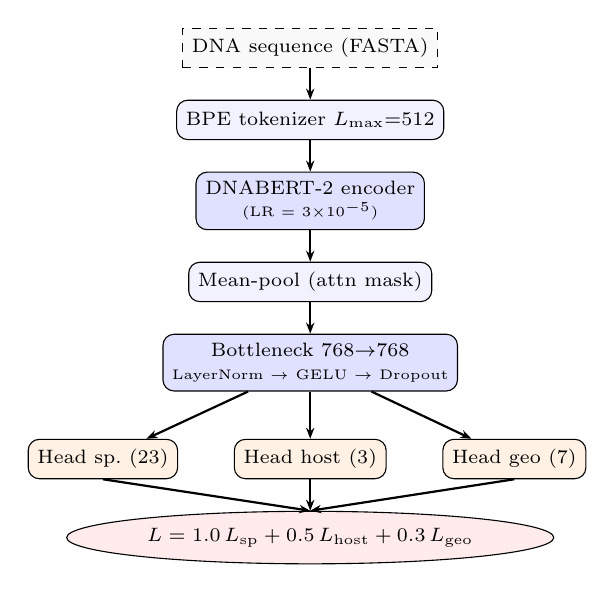
\begin{tikzpicture}[
  node distance=4mm and 6mm,
  every node/.style={font=\scriptsize},
  block/.style={rectangle, draw, rounded corners, minimum width=2.2cm,
                minimum height=5mm, align=center, fill=blue!5},
  data/.style={rectangle, draw, dashed, minimum width=2.2cm,
               minimum height=5mm, align=center, fill=gray!5},
  head/.style={rectangle, draw, rounded corners, minimum width=1.7cm,
               minimum height=5mm, align=center, fill=orange!10},
  loss/.style={ellipse, draw, minimum width=1.6cm, minimum height=5mm,
               align=center, fill=red!8},
  arrow/.style={-{Stealth[length=1.4mm]}, thick},
]
\node[data] (seq) {DNA sequence (FASTA)};
\node[block, below=of seq] (tok) {BPE tokenizer $L_{\max}{=}512$};
\node[block, below=of tok, fill=blue!12] (enc)
      {DNABERT-2 encoder \\ \tiny (LR = $3{\times}10^{-5}$)};
\node[block, below=of enc] (pool) {Mean-pool (attn mask)};
\node[block, below=of pool, fill=blue!12] (bot)
      {Bottleneck $768{\to}768$ \\ \tiny LayerNorm $\to$ GELU $\to$ Dropout};
\node[head, below left=6mm and -2mm of bot]  (hsp)  {Head sp.\ (23)};
\node[head, below=6mm of bot]                (hho)  {Head host (3)};
\node[head, below right=6mm and -2mm of bot] (hge)  {Head geo (7)};
\node[loss, below=of hho] (loss) {$L = 1{.}0\,L_{\text{sp}} + 0{.}5\,L_{\text{host}} + 0{.}3\,L_{\text{geo}}$};
\draw[arrow] (seq)  -- (tok);
\draw[arrow] (tok)  -- (enc);
\draw[arrow] (enc)  -- (pool);
\draw[arrow] (pool) -- (bot);
\draw[arrow] (bot)  -- (hsp);
\draw[arrow] (bot)  -- (hho);
\draw[arrow] (bot)  -- (hge);
\draw[arrow] (hsp.south) -- (loss.north);
\draw[arrow] (hho.south) -- (loss.north);
\draw[arrow] (hge.south) -- (loss.north);
\end{tikzpicture}
\caption{HantaBERT computation flow. Dark-blue components are trained with
the encoder \emph{learning rate} ($3\!\times\!10^{-5}$); light-blue and
orange components with an LR ten times larger.}
\label{fig:flow}
\end{figure}

\subsection{Multi-Task \emph{Loss} Function}

The overall \emph{loss} is a linear combination of three class-weighted
\emph{cross-entropy} terms:
\[
L \;=\; \lambda_{\text{sp}}\,L_{\text{sp}}
     \,+\, \lambda_{\text{host}}\,L_{\text{host}}
     \,+\, \lambda_{\text{geo}}\,L_{\text{geo}},
\]
with $\lambda_{\text{sp}}{=}1{.}0$, $\lambda_{\text{host}}{=}0{.}5$,
and $\lambda_{\text{geo}}{=}0{.}3$. The weights reflect relative
priority: species is the primary task with the cleanest supervision, while
geography has the lowest signal-to-noise ratio.

\subsection{Training Strategy}

The training configuration is summarized in Table~\ref{tab:hyper}. The
pre-trained \emph{encoder} is given a learning rate ten times smaller than
the new layers (\emph{bottleneck} and heads). Because the 512-token
\emph{full attention} of DNABERT-2 cannot fit a \emph{batch} of 16 on a
\emph{consumer-grade} GPU, an effective \emph{batch size} of 16 is reached
via $\text{BATCH\_SIZE}{=}4$ and $\text{GRAD\_ACCUM\_STEPS}{=}4$. In
addition, the \texttt{attention\_probs\_dropout\_prob} parameter is set to
$0{.}1$ to force the standard PyTorch \emph{attention} path, avoiding the
DNABERT-2 Triton \emph{kernel} that exceeds the \emph{shared memory}
limit.

\begin{table}[t]
\centering
\caption{Main training hyperparameters.}
\label{tab:hyper}
\begin{tabular}{ll}
\toprule
\textbf{Parameter} & \textbf{Value} \\
\midrule
Backbone & \texttt{zhihan1996/DNABERT-2-117M} \\
Max token length & 512 BPE \\
\emph{Batch size} & 4 ($\times$ 4 \emph{grad accum} = effective 16) \\
LR encoder / heads & $3{\times}10^{-5}$ / $3{\times}10^{-4}$ \\
Optimizer & AdamW, $\beta=(0{.}9,0{.}999)$, $\text{wd}=0{.}01$ \\
\emph{Warmup} / total epochs & 200 linear steps / 10 \\
\emph{Mixed precision} & AMP fp16 \\
\emph{Grad clipping} & 1{.}0 (\emph{global norm}) \\
$\lambda_{\text{sp/host/geo}}$ & $1{.}0/0{.}5/0{.}3$ \\
\bottomrule
\end{tabular}
\end{table}

\subsection{Web Interface for Inference}\label{sec:webui}

To make the model ready for use by non-programmer researchers, a public
web interface was developed. The \emph{backend} (\texttt{HantaBERT-API})
wraps the \texttt{MultiTaskHantaBERT} \emph{checkpoint} behind a
FastAPI + Uvicorn service, packaged as a Docker \emph{container} based on
\texttt{python:3.11-slim}, and \emph{deployed} at
\texttt{hantabert-api.faizath.com}. The \emph{frontend}
(\texttt{HantaBERT-Web}) is a set of pure static HTML/CSS/JavaScript files
with no JS \emph{framework}; the interactive world map for geographic
origin is drawn using the D3 and TopoJSON libraries loaded from a CDN.

Users can paste a raw DNA/RNA sequence or upload a FASTA file; the $U$
bases in RNA input are automatically converted to $T$ before BPE
tokenization, and the system displays a warning when a sequence exceeds
512 tokens and is therefore truncated. The number of \emph{top-N} results
(1 to 23) can be configured per task, complete with an expandable
\emph{confidence score}. Figure~\ref{fig:webui} shows the system output
for a 224 bp test sequence run directly on the interface.

\begin{figure}[t]
\centering
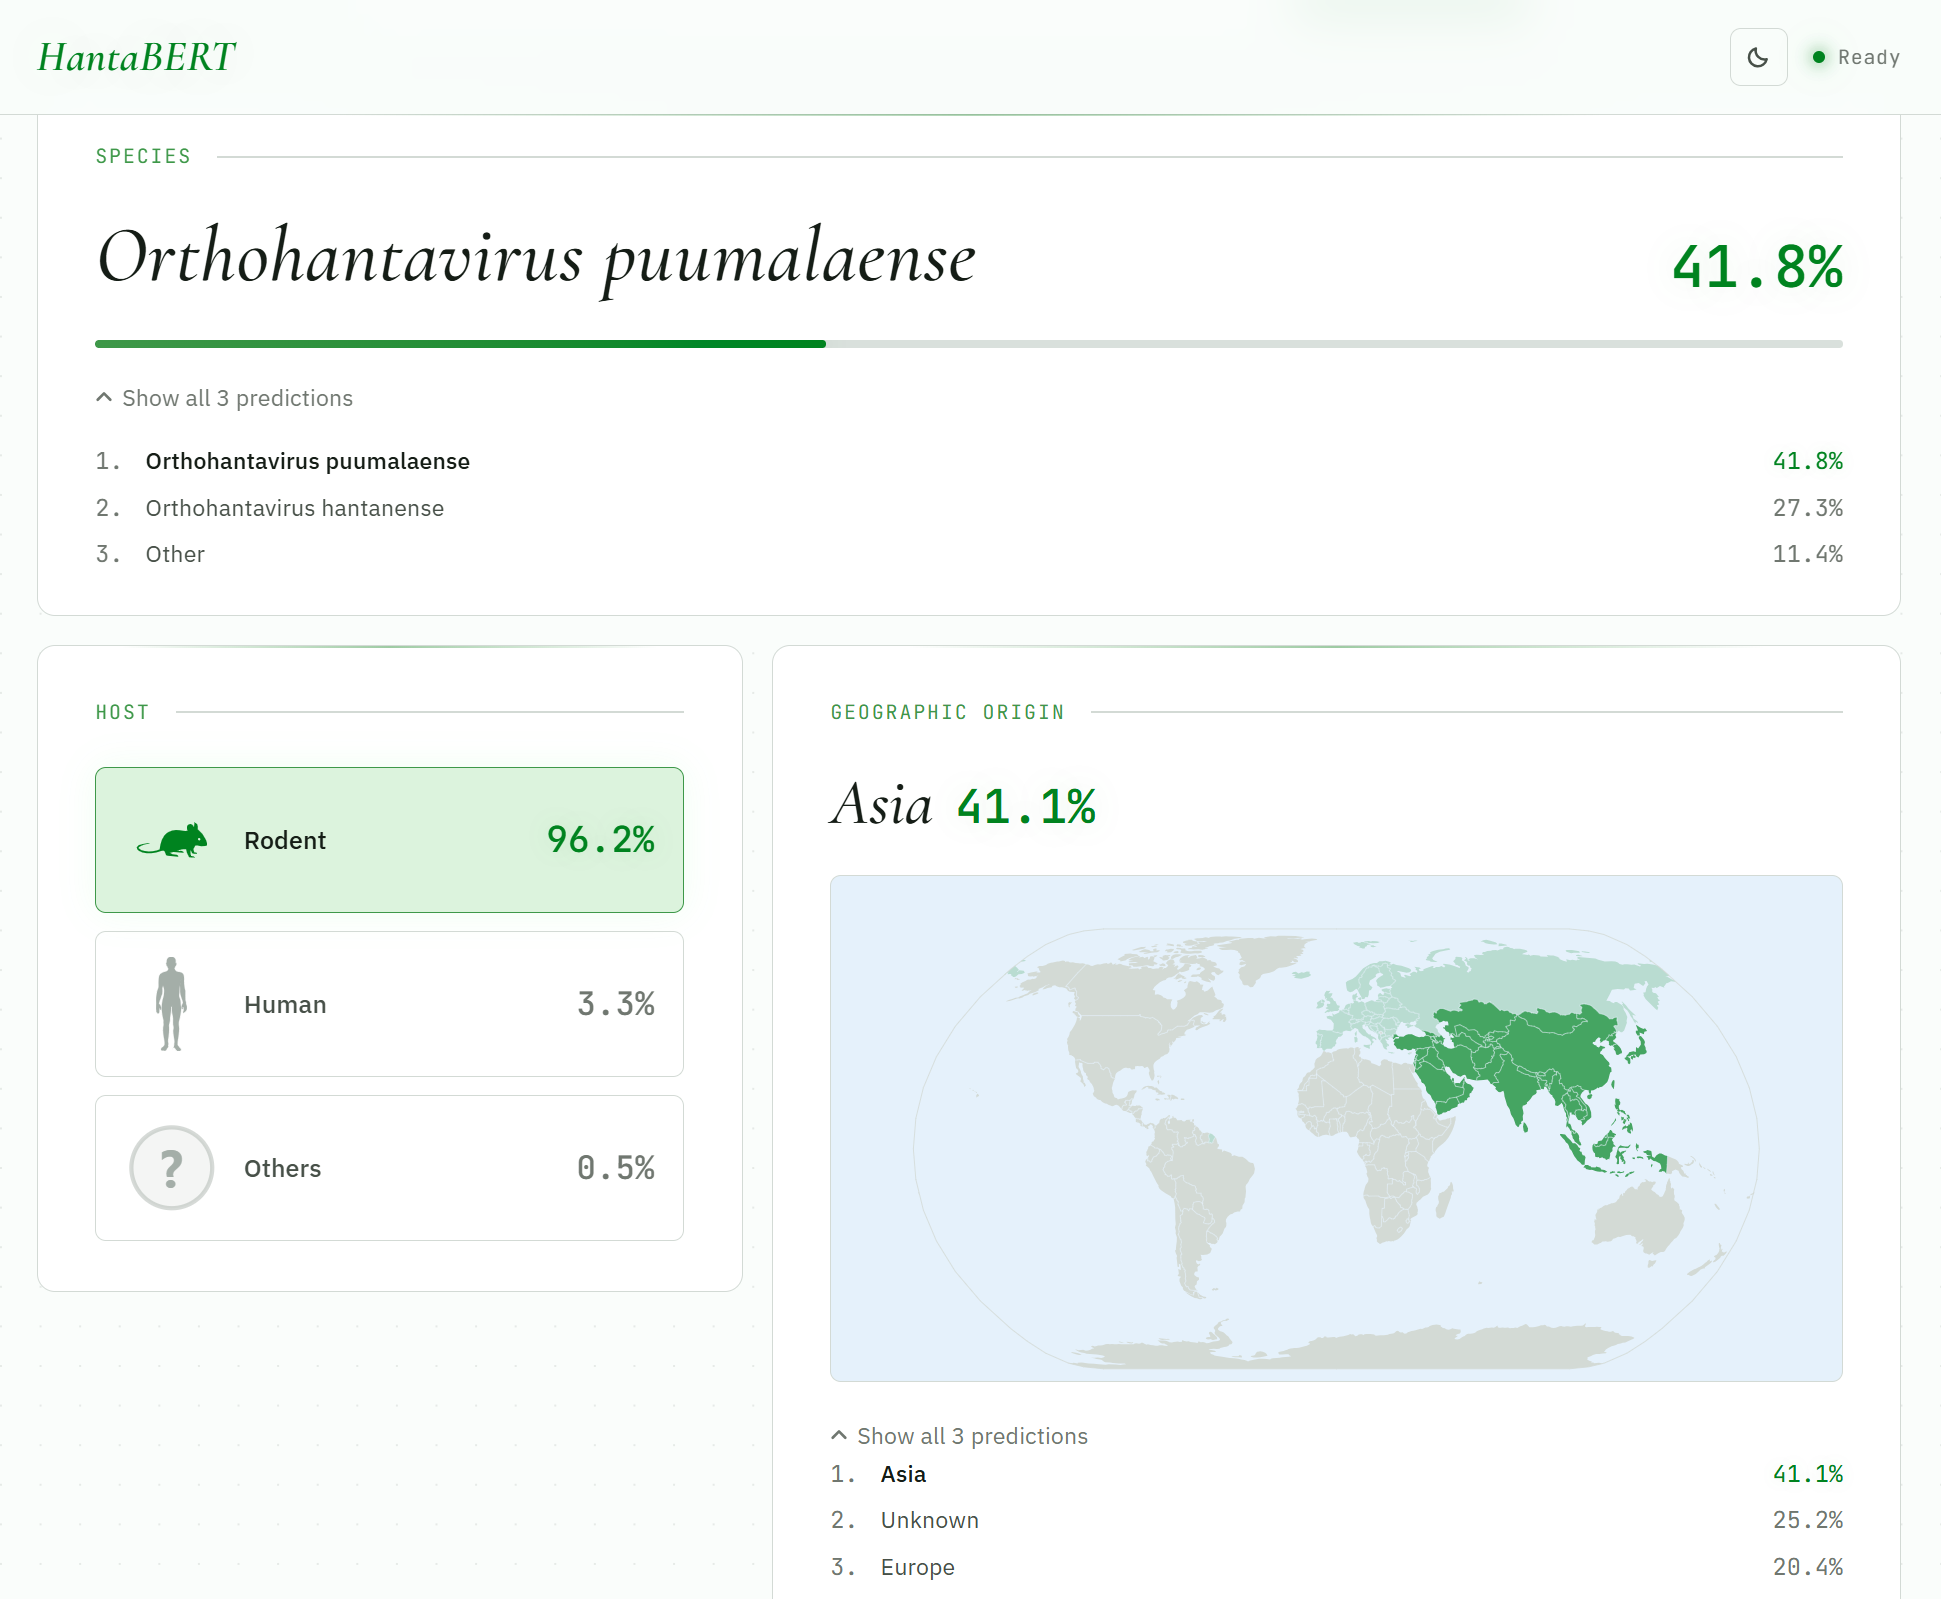
\includegraphics[width=\linewidth]{website-interface.png}
\caption{Screenshot of the HantaBERT web interface for a 224 bp test
  sequence \texttt{ATGAAAGACCTTCTGAAG\ldots GAGAAGCTGGAG}. The
  \emph{top-1} predictions: \emph{Orthohantavirus puumalaense}
  ($41{.}8\%$), host \emph{Rodent} ($96{.}2\%$), and geographic region
  Asia ($41{.}1\%$). The \emph{top-3} probabilities can be expanded on
  each task card; the geography result is visualized on an interactive
  world map.}
\label{fig:webui}
\end{figure}

\subsection{Code and Data Availability}

All artifacts are released openly under the GitHub organization
\url{https://github.com/HantaBERT}, comprising three repositories:
(i) \texttt{HantaBERT}: the \emph{preprocess}, \emph{train},
\emph{evaluate}, \emph{visualize} code, hyperparameters, and model
\emph{checkpoint}; (ii) \texttt{HantaBERT-API}: the FastAPI inference
service together with its \emph{Dockerfile}; (iii) \texttt{HantaBERT-Web}:
the static \emph{frontend} files. Each repository includes a
\texttt{requirements.txt}/\texttt{README} listing the tested package
versions and a step-by-step reproduction guide. In addition, a link to a
recorded presentation video is provided at
\url{https://youtu.be/4Ia0FM7iYb4} and the presentation slides can be
accessed at \url{https://canva.link/33nwtodm1si8nxw}.

% =============================================================================
\section{Results and Discussion}\label{sec:results}
% =============================================================================

\subsection{Training Progress}

Table~\ref{tab:hist} shows the progress at each epoch on the validation
set. After 10 epochs, \emph{val\_loss} dropped from $2{.}443$ to $0{.}797$
and validation accuracy reached $96{.}7\%$ (species), $91{.}4\%$ (host),
$80{.}5\%$ (geography). The species task saturated the fastest, consistent
with its cleanest supervision and a class count that makes the
discriminative signal rich. The curves in Figure~\ref{fig:curves} show the
training-validation \emph{loss} gap shrinking over epochs with no clear
sign of overfitting.

\begin{table}[t]
\centering
\caption{Training progress on the validation set (10 epochs).}
\label{tab:hist}
\begin{tabular}{cccccc}
\toprule
\textbf{Ep} & \textbf{$L_{\text{tr}}$} & \textbf{$L_{\text{val}}$} &
\textbf{Sp.} & \textbf{Host} & \textbf{Geo} \\
\midrule
1  & 3{.}024 & 2{.}443 & 78{.}9\% & 72{.}8\% & 72{.}3\% \\
3  & 1{.}034 & 1{.}195 & 92{.}9\% & 83{.}1\% & 74{.}1\% \\
5  & 0{.}634 & 1{.}150 & 94{.}0\% & 87{.}1\% & 77{.}6\% \\
7  & 0{.}452 & 0{.}869 & 96{.}5\% & 90{.}4\% & 78{.}1\% \\
9  & 0{.}336 & 0{.}818 & 96{.}3\% & 91{.}4\% & 80{.}3\% \\
\textbf{10} & \textbf{0{.}307} & \textbf{0{.}797} &
\textbf{96{.}7\%} & \textbf{91{.}4\%} & \textbf{80{.}5\%} \\
\bottomrule
\end{tabular}
\end{table}

\begin{figure}[t]
\centering
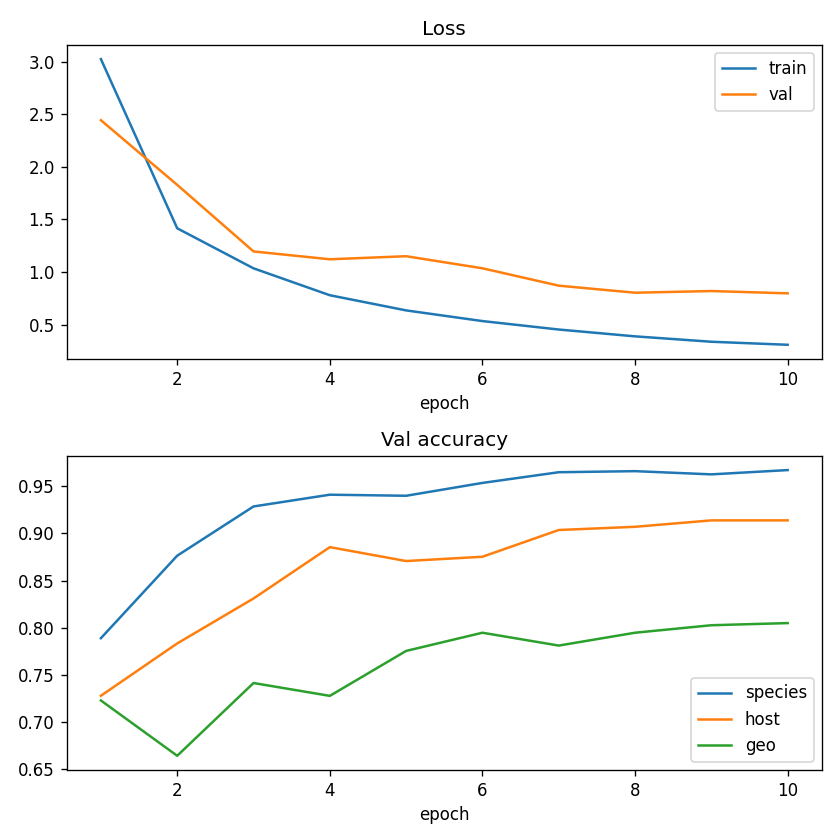
\includegraphics[width=\linewidth]{training_curves.png}
\caption{\emph{Loss} curves (top) and per-task validation accuracy
(bottom) over 10 epochs.}
\label{fig:curves}
\end{figure}

\subsection{Evaluation on the Test Set}

Table~\ref{tab:test} summarizes the test-set accuracy for two evaluation
paths: the post-training neural heads and an SVM-RBF \emph{baseline}
($C\!=\!10$, \emph{balanced} classes) over the frozen and standardized
\emph{bottleneck embedding}. The purpose of this baseline is to measure
the quality of the \emph{embedding} in isolation (not to beat the neural
heads) and to answer \textbf{RQ2}: if a simple SVM-RBF can achieve high
accuracy over $\mathbf{z}$, it means the \emph{bottleneck} has indeed
mapped the sequences into a space whose classes are non-linearly
separable.

\begin{table}[t]
\centering
\caption{Accuracy on the test set.}
\label{tab:test}
\begin{tabular}{lc}
\toprule
\textbf{Task} & \textbf{Neural head} \\
\midrule
Species (23) & \textbf{96{.}7\%} \\
Host (3)     & \textbf{91{.}4\%} \\
Geography (7) & \textbf{80{.}5\%} \\
\bottomrule
\end{tabular}
\end{table}

\subsection{Error Analysis and Biological Context}

Figure~\ref{fig:cm-species} shows the \emph{confusion matrix} for the
species task; dominant \emph{lineages} (e.g.\ \emph{O.\ seoulense},
\emph{O.\ puumalaense}) are predicted with high accuracy, and the errors
concentrate on the \emph{Other} class, which is an aggregate of rare
lineages, a direct consequence of the $<\!30$-sample threshold.

\begin{figure}[t]
\centering
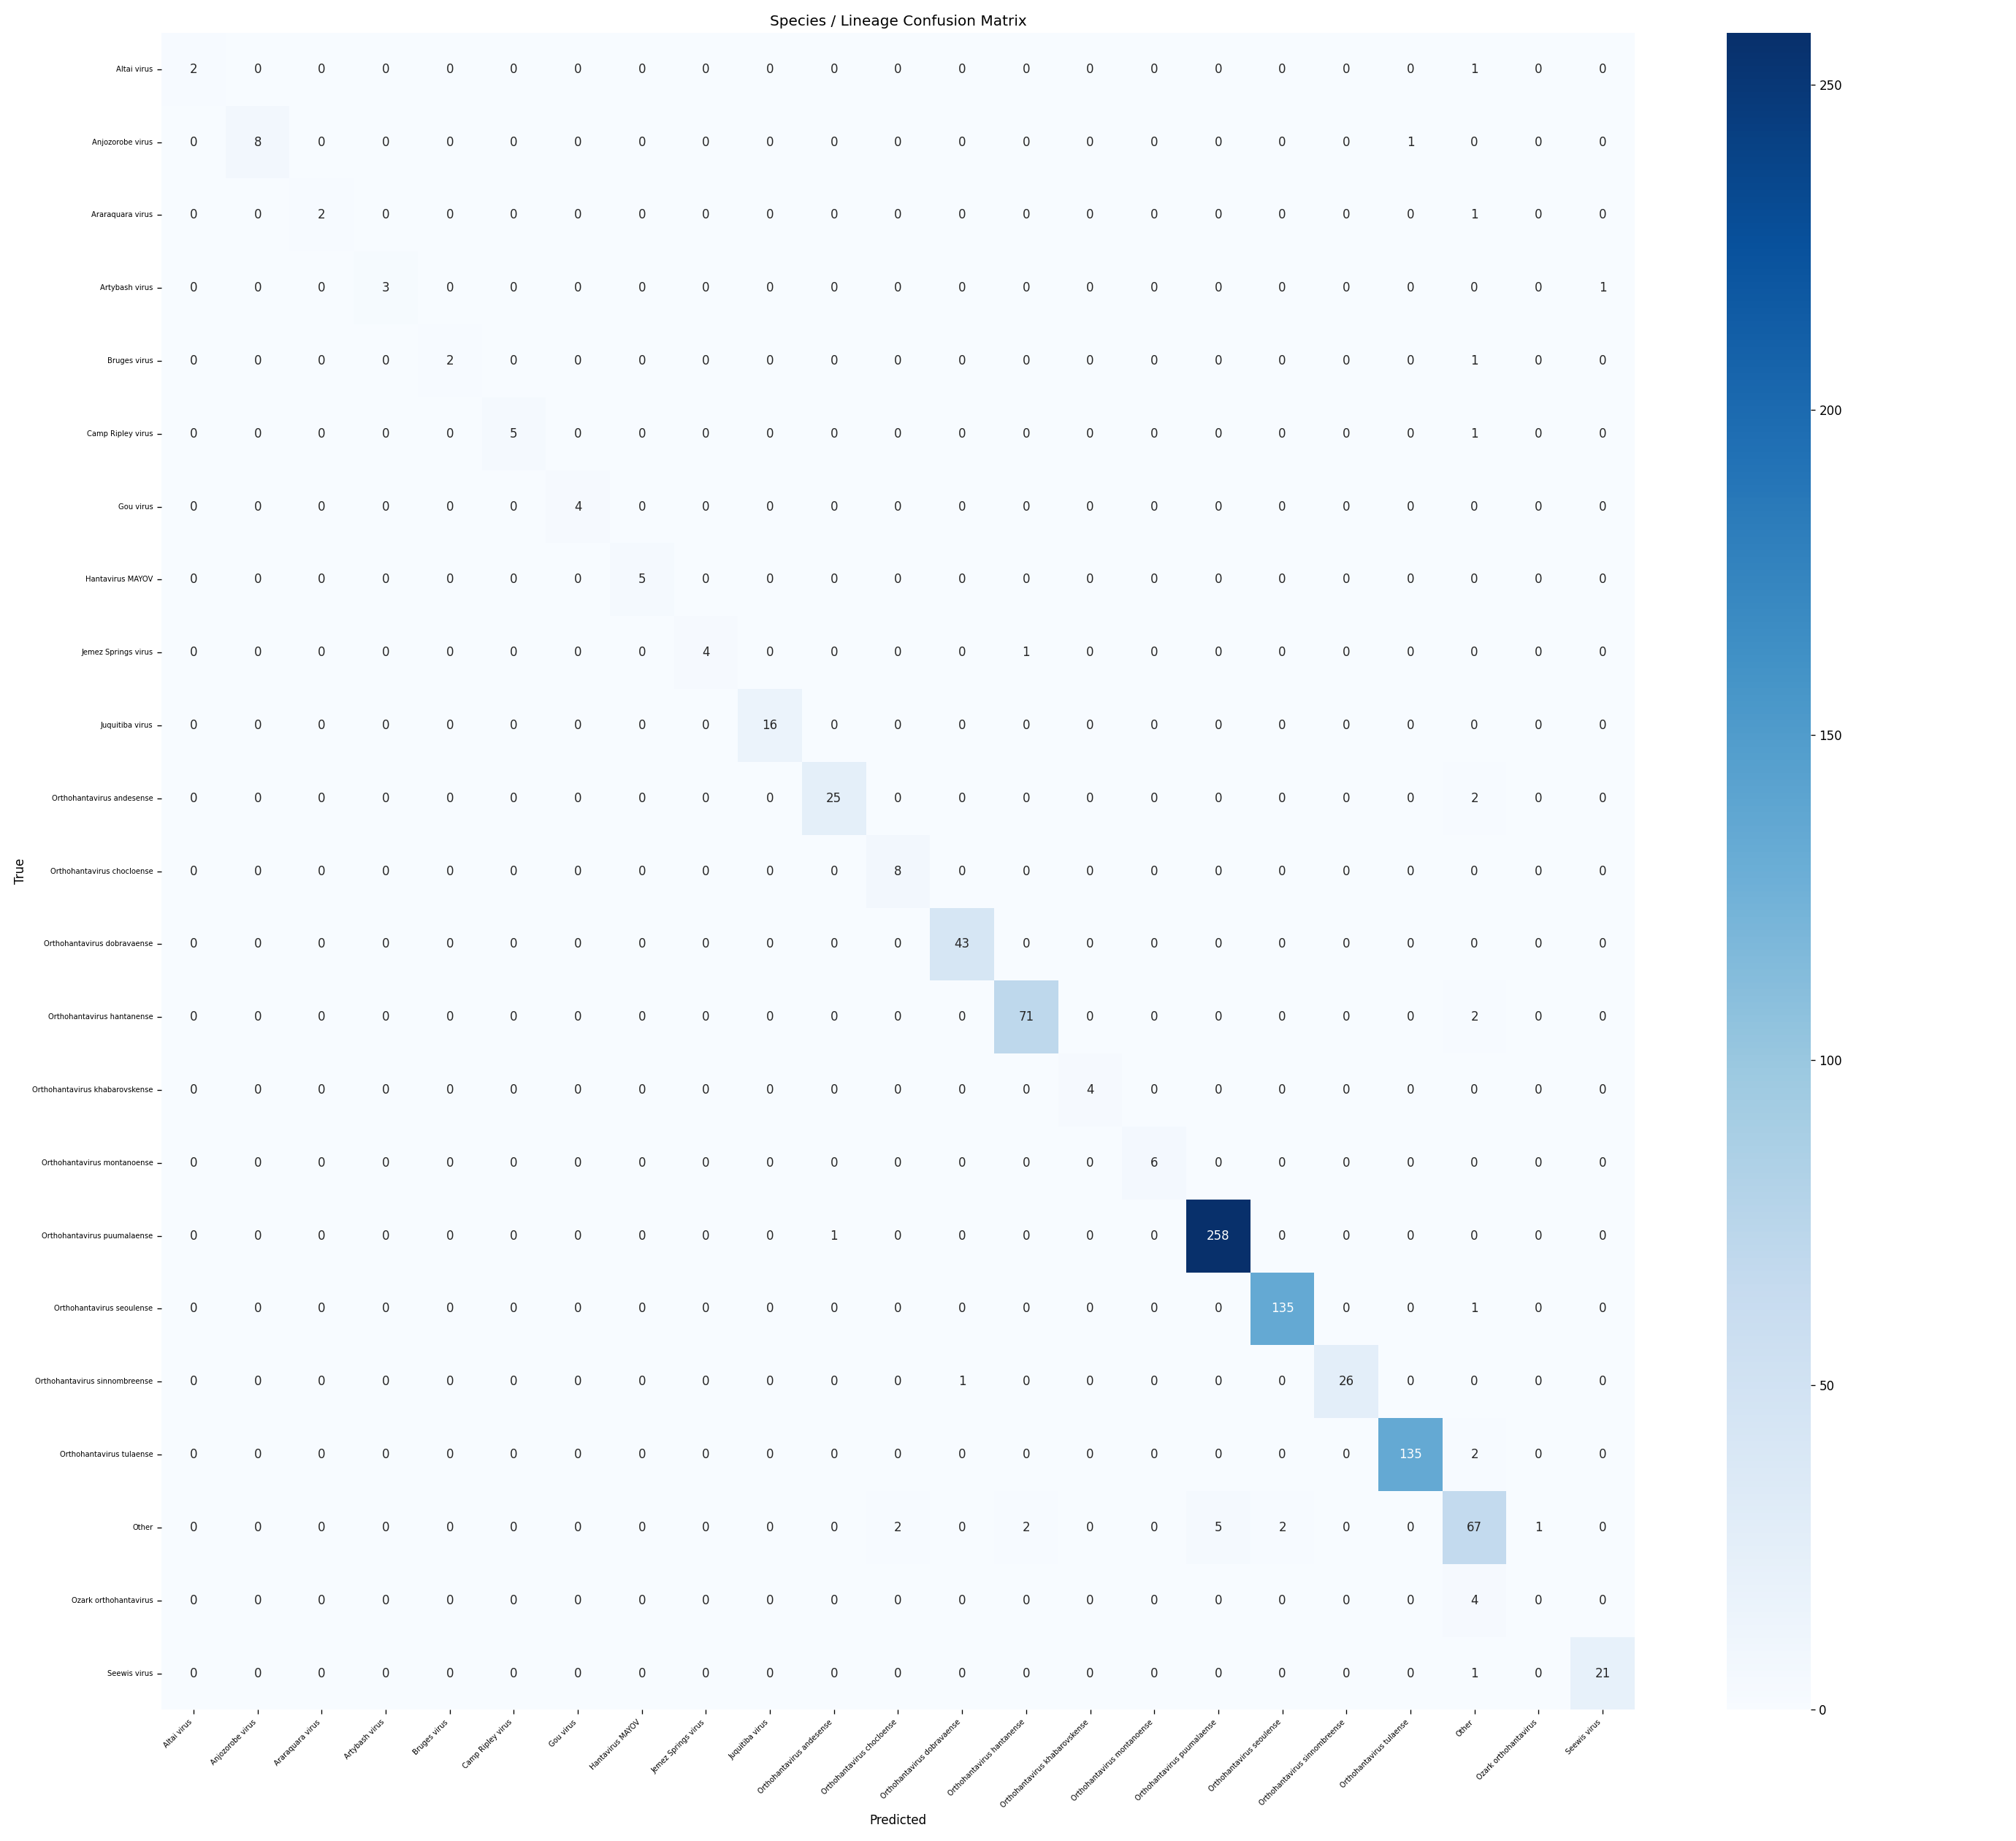
\includegraphics[width=\linewidth]{cm_species.png}
\caption{\emph{Confusion matrix} for species classification on the test
set.}
\label{fig:cm-species}
\end{figure}

In the host task, most errors are confusions between \emph{Rodent} and
\emph{Others}, which is reasonable because some hantaviruses
(e.g.\ \emph{Thottimvirus}) are also isolated from non-rodent
\emph{Insectivora} (bats, shrews). In the geography task, errors
concentrate on \emph{cosmopolitan} lineages: the Seoul virus carried by
\emph{Rattus norvegicus} is found on every continent following the
distribution of its host rat, so the continent label is not always
deterministic from the sequence; the $80{.}5\%$ accuracy is likely an
upper bound close to the inherent ambiguity of that label.

\subsection{UMAP Visualization and Phylogenetic Substructure}

To answer \textbf{RQ2} and \textbf{RQ3}, UMAP
($n_{\text{neighbors}}{=}20$, $\text{min\_dist}{=}0{.}1$,
\emph{cosine} metric) was applied to the \emph{bottleneck embedding} of
all sequences; a variant with $n_{\text{neighbors}}{=}15$,
$\text{min\_dist}{=}0{.}05$ was used for the intra-species plots.
Figure~\ref{fig:umap-all} shows the \emph{embedding} forming separate
clusters per \emph{lineage}, a result that is not explicitly supervised by
any \emph{clustering} objective.

\begin{figure}[t]
\centering
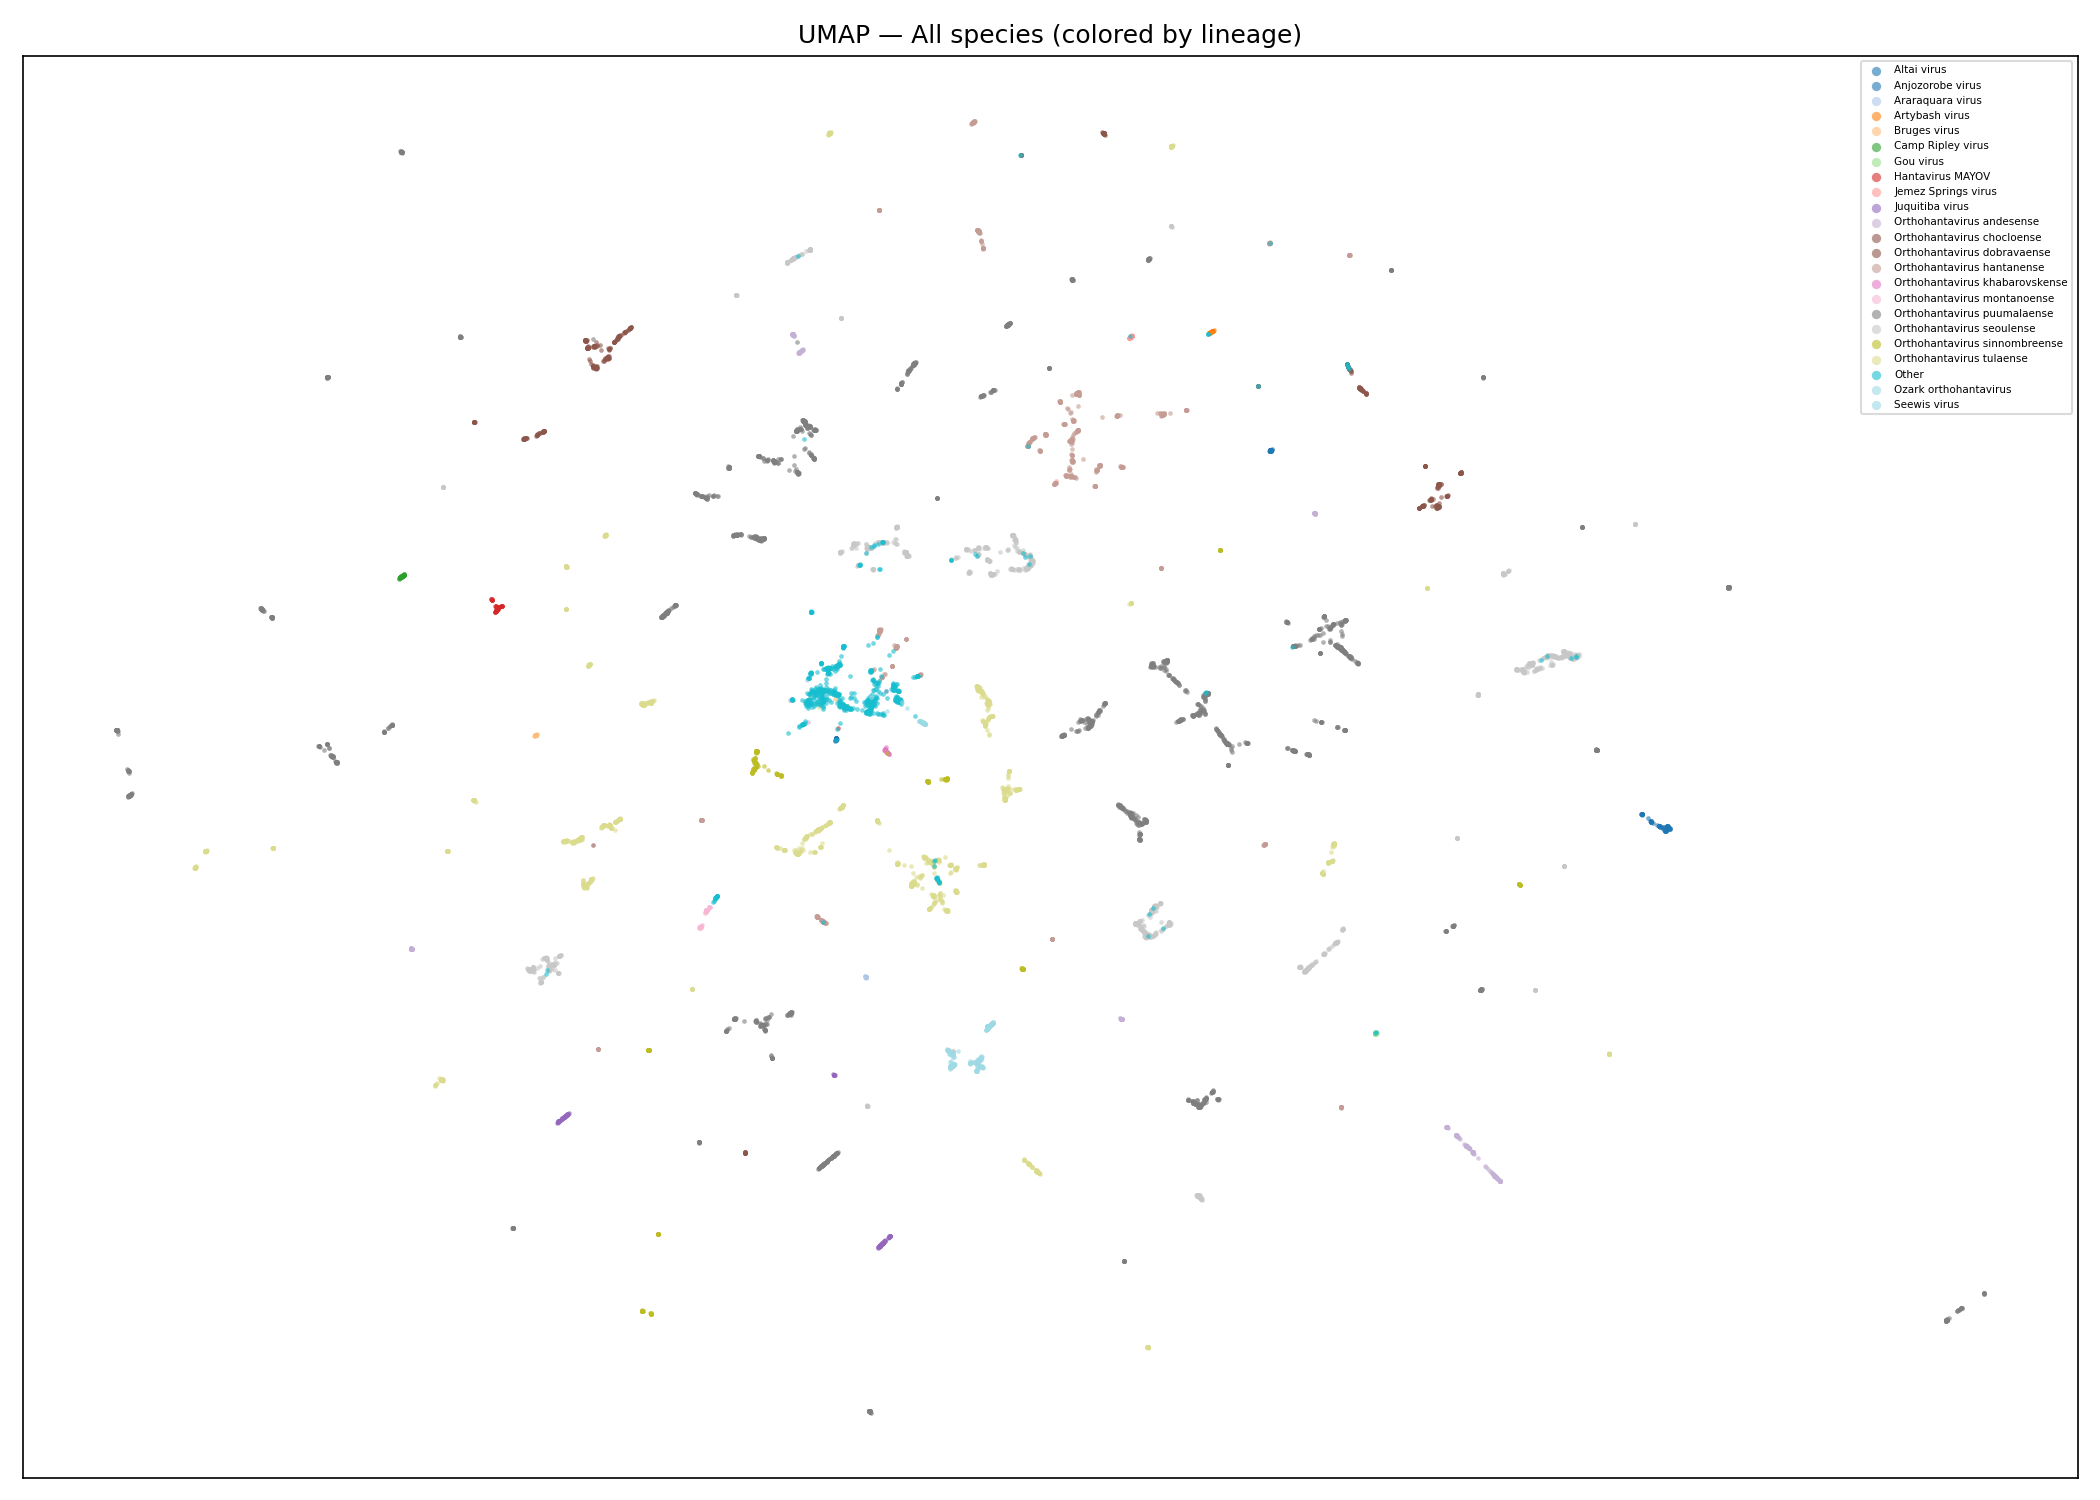
\includegraphics[width=\linewidth]{umap_all_species.png}
\caption{UMAP projection of 8{,}822 sequences colored by lineage.}
\label{fig:umap-all}
\end{figure}

The intra-species plots (Figures~\ref{fig:umap-seoul}
and~\ref{fig:umap-puumala}) reveal an interesting phenomenon: the
\emph{embedding} groups sequences by \textbf{genome segment}
($S$/$M$/$L$) even though the segment is never a supervision target. This
is consistent with hantavirus biology: the three segments encode proteins
with different selective pressures and nucleotide content: N (segment S)
is highly \emph{conserved}, Gn/Gc (segment M) undergo \emph{positive
selection} at envelope antigenic sites, and RdRp (segment L) preserves the
active polymerase motifs. These differences in \emph{di-} and
\emph{tri-nucleotide} composition are detected by the DNABERT-2 BPE
\emph{tokenizer} and manifest in the \emph{embedding} as cluster
separation, answering \textbf{RQ3}: the model has implicitly mapped the
structural information of the hantavirus genome.

\begin{figure}[t]
\centering
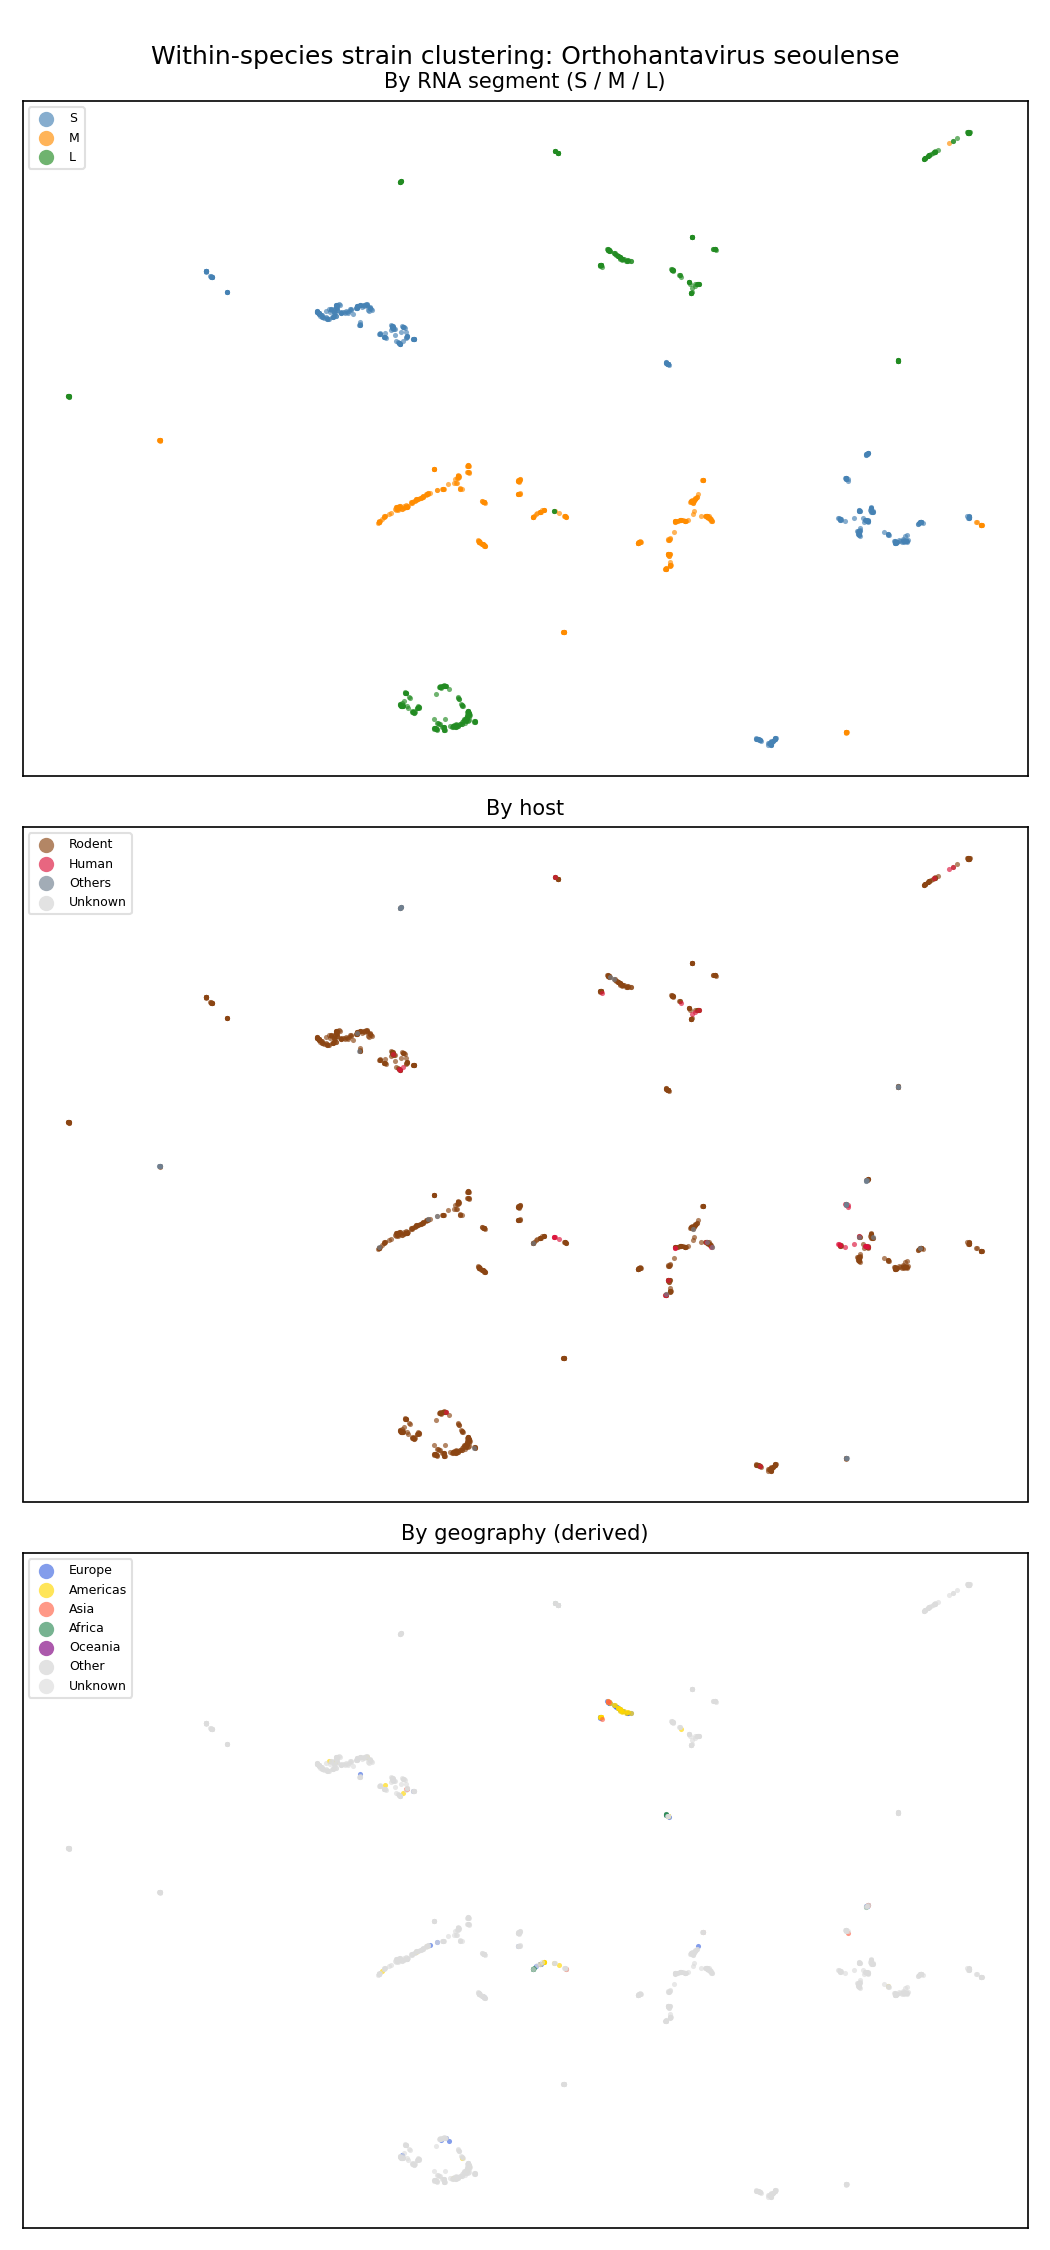
\includegraphics[width=\linewidth,height=0.6\textheight,keepaspectratio]{umap_Orthohantavirus_seoulense.png}
\caption{Intra-species UMAP of \emph{O.\ seoulense} (top-to-bottom:
segment / host / geography).}
\label{fig:umap-seoul}
\end{figure}

\begin{figure}[t]
\centering
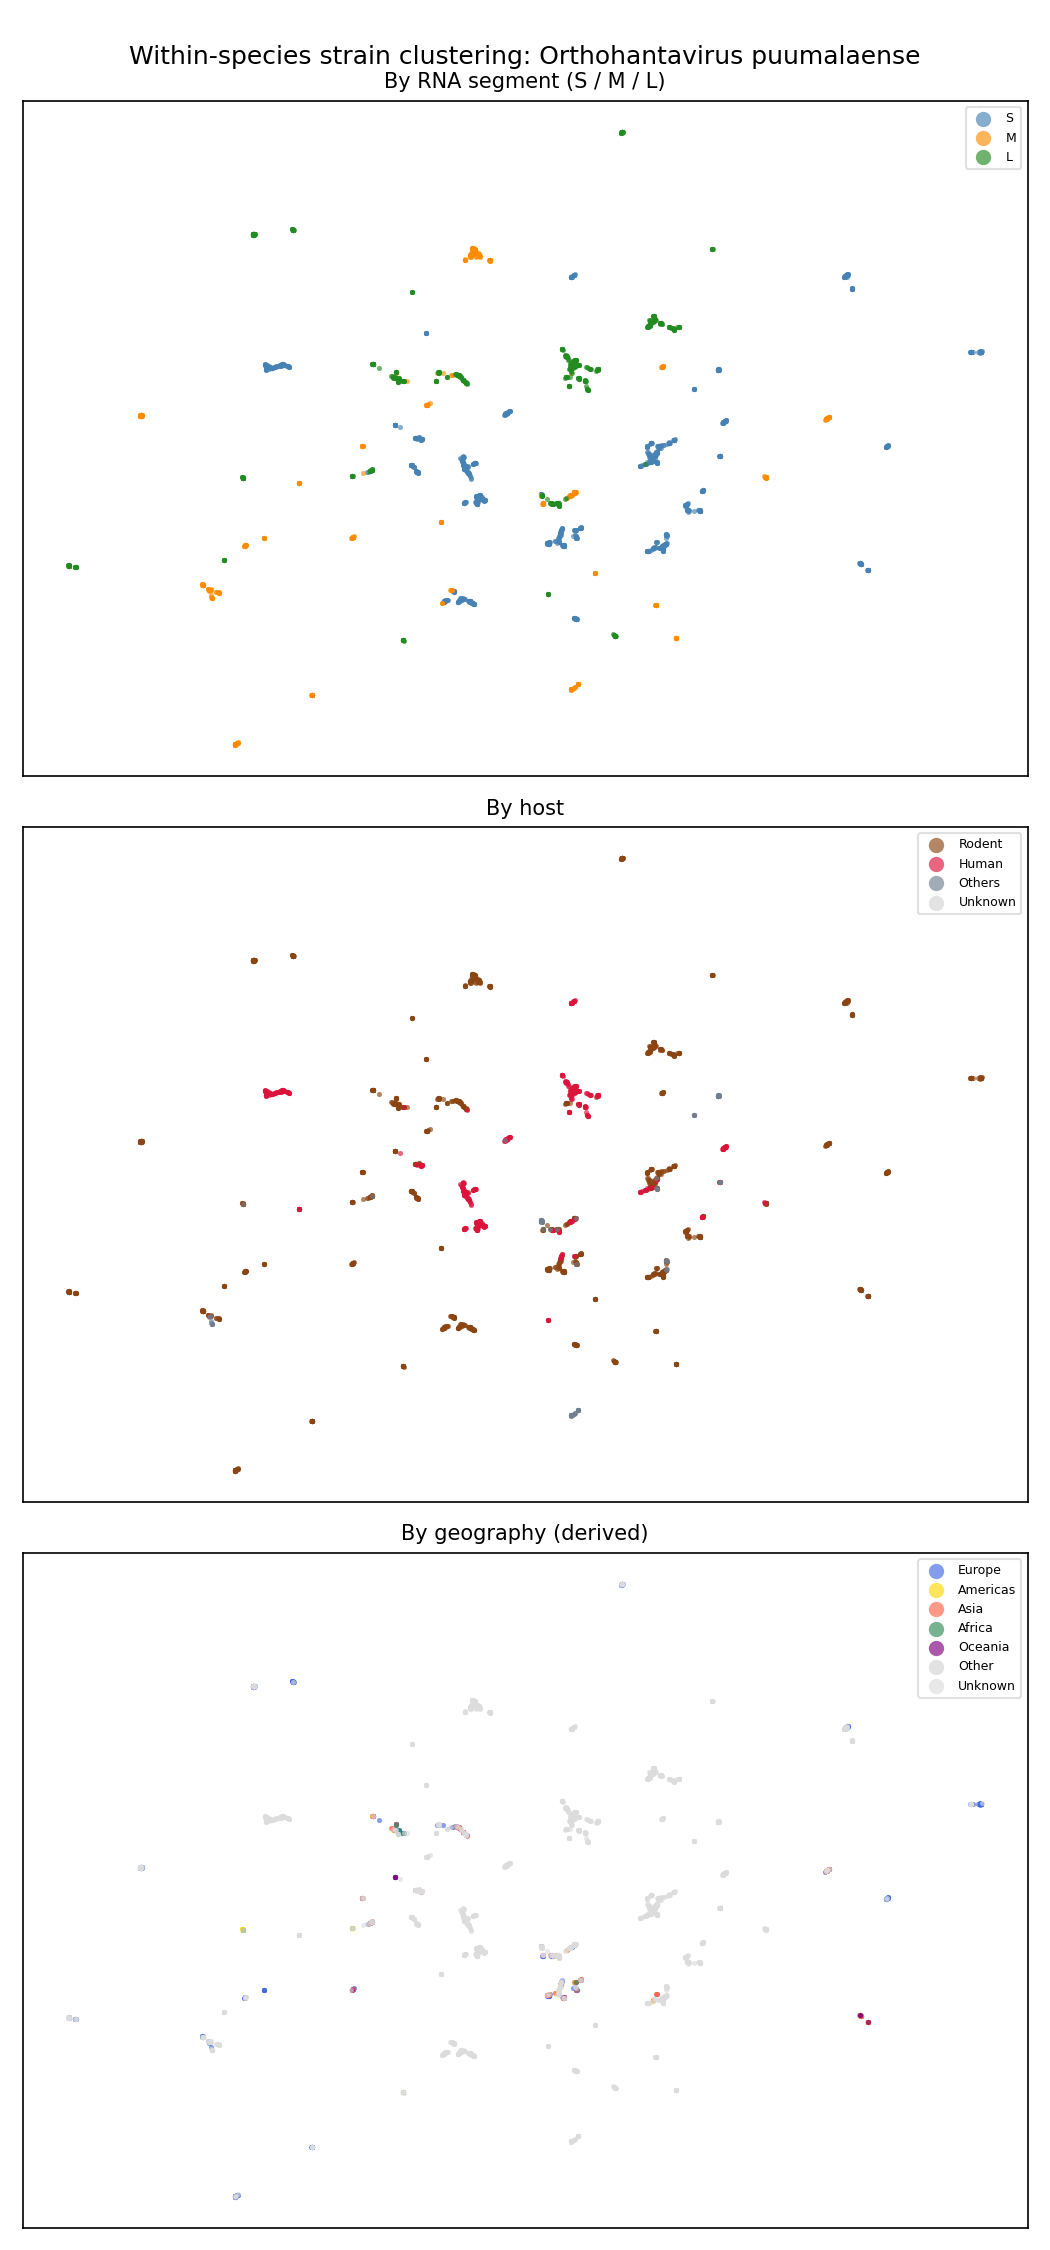
\includegraphics[width=\linewidth,height=0.6\textheight,keepaspectratio]{umap_Orthohantavirus_puumalaense.png}
\caption{Intra-species UMAP of \emph{O.\ puumalaense} (top-to-bottom:
segment / host / geography).}
\label{fig:umap-puumala}
\end{figure}

% =============================================================================
\section{Conclusion}\label{sec:conclusion}
% =============================================================================

This study presents HantaBERT, a multi-task model obtained by
\emph{fine-tuning} DNABERT-2 to classify the species, host, and geographic
origin of hantavirus sequences in a single \emph{forward pass}. The shared
\emph{bottleneck} scheme, the weighted multi-task \emph{loss}, and the
memory-friendly training strategy (AMP fp16, \emph{grad accum},
differential LR) yield 96{.}7\%/91{.}4\%/80{.}5\% accuracy on a held-out
test set, answering \textbf{RQ1} affirmatively. The 768-d
\emph{embedding} that emerges from training not only forms lineage
clusters (\textbf{RQ2}) but also substructure per genome segment
($S$/$M$/$L$) consistent with viral biology (\textbf{RQ3}). Objectively,
this contribution provides a compact computational basis for triaging new
hantavirus sequences: multi-attribute classification + a
visualization-ready representation with a single model. Complementing the
\emph{engineering} contribution, the model is \emph{deployed} behind a
public web interface (FastAPI + static HTML/JS frontend) that accepts
DNA/RNA sequences or FASTA files and returns probabilistic predictions per
task together with an interactive geographic map.

Directions for future work: (i) extending the context beyond 512 tokens so
that long $L$ segments are not truncated; (ii) a probability calibration
head (\emph{temperature}/\emph{Platt scaling}) for reliable uncertainty
estimation in surveillance; (iii) a cross-genome-segment \emph{ensemble}
when all three segments of one isolate are available; (iv) exploring
DNABERT-S as an alternative \emph{backbone} because its pre-training
objective is \emph{species-aware}.

% =============================================================================
\begin{thebibliography}{99}

\bibitem{Zhou2023DNABERT2}
Z. Zhou, Y. Ji, W. Li, P. Dutta, R. Davuluri, and H. Liu,
``DNABERT-2: Efficient foundation model and benchmark for multi-species
genome,'' \emph{arXiv preprint} arXiv:2306.15006, 2023.

\bibitem{Zhou2024DNABERTS}
Z. Zhou, W. Wu, H. Ho, J. Wang, L. Shi, R. V. Davuluri, Z. Wang, and H. Liu,
``DNABERT-S: Learning species-aware DNA embedding with genome foundation
models,'' \emph{arXiv preprint} arXiv:2402.08777, 2024.

\bibitem{Ji2021DNABERT}
Y. Ji, Z. Zhou, H. Liu, and R. V. Davuluri,
``DNABERT: pre-trained bidirectional encoder representations from
transformers model for DNA-language in genome,''
\emph{Bioinformatics}, vol. 37, no. 15, pp. 2112-2120, 2021.

\bibitem{Devlin2019BERT}
J. Devlin, M.-W. Chang, K. Lee, and K. Toutanova,
``BERT: Pre-training of deep bidirectional transformers for language
understanding,'' in \emph{Proc. NAACL-HLT}, 2019, pp. 4171-4186.

\bibitem{Caruana1997MTL}
R. Caruana, ``Multitask learning,'' \emph{Machine Learning}, vol. 28,
pp. 41-75, 1997.

\bibitem{McInnes2018UMAP}
L. McInnes, J. Healy, and J. Melville,
``UMAP: Uniform manifold approximation and projection for dimension
reduction,'' \emph{arXiv preprint} arXiv:1802.03426, 2018.

\bibitem{Wolf2020Transformers}
T. Wolf \emph{et al.},
``Transformers: State-of-the-art natural language processing,'' in
\emph{Proc. EMNLP: System Demonstrations}, 2020, pp. 38-45.

\bibitem{Paszke2019PyTorch}
A. Paszke \emph{et al.},
``PyTorch: An imperative style, high-performance deep learning library,''
in \emph{Proc. NeurIPS}, 2019.

\bibitem{Pedregosa2011Sklearn}
F. Pedregosa \emph{et al.},
``Scikit-learn: Machine learning in Python,''
\emph{J. Mach. Learn. Res.}, vol. 12, pp. 2825-2830, 2011.

\bibitem{Loshchilov2019AdamW}
I. Loshchilov and F. Hutter,
``Decoupled weight decay regularization,'' in \emph{Proc. ICLR}, 2019.

\end{thebibliography}

\end{document}
